\chapter{Diagrama de classes}

A figura \ref{fig:fullDiagram} é o diagrama de classes detalhado do protótipo.
\begin{figure}[H]
    \centering
    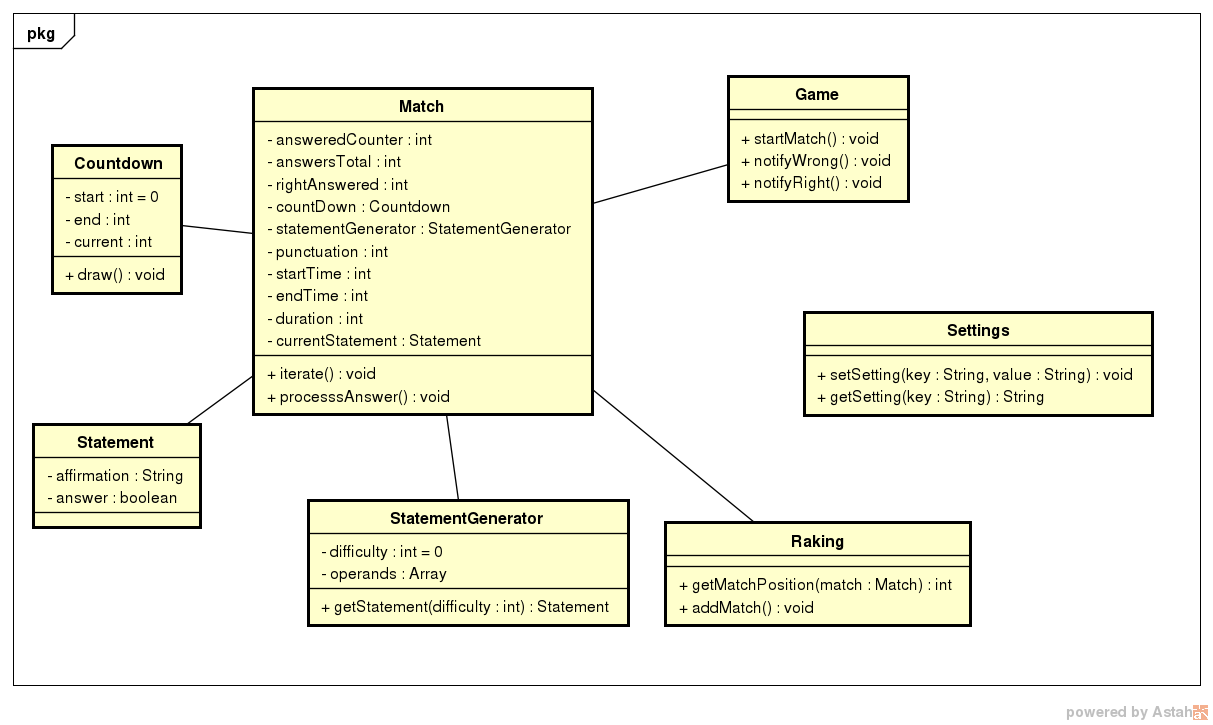
\includegraphics[width=0.8\textwidth,natwidth=610,natheight=642]{ClassesFullView.png}
	\caption{Diagrama de classes completo}
    \label{fig:fullDiagram}
\end{figure}

\chapter{Bibliotecas relevantes no desenvolvimento de jogos Web}

Desta parte em diante serão tratadas tecnologias associadas ao
desenvolvimento de jogos Web que não compõem as tecnologias centrais
da plataforma. Sendo assim, limitações nestas tecnologias não
caracterizam limitações na plataforma Web e por isso não foram tratadas
na parte principal do texto. Entretanto, estas tecnologias são de grande relevância para
desenvolvedores interessados em criar jogos para a Web.

A quantidade de ferramentas Web a disposição dos usuários é
enorme. Segundo \citet{html5mostwanted} desenvolvedores da Web são
geralmente de mente aberta e criaram uma quase infinita variedade de
bibliotecas e frameworks pela internet. Sabendo disso, é uma tarefa
praticamente impossível ter habilidade em todas as ferramentas
existentes. Entretanto, é importante que os desenvolvedores ao menos
conheçam as ferramentas mais importantes disponíveis para que, no
momento necessário, saibam qual aprender. Todavia, \citet{creatingFun}
ressalta a importância de sermos moderados quanto a escolha de
bibliotecas no contexto Web multiplataforma.

\begin{quote}
Muitos desenvolvedores da Web utilizam bibliotecas como jQuery e o
Prototype de modo a se verem livres de ter que lidar com
partes triviais do desenvolvimento Web, como selecionar e
manipular elementos do DOM. Muitas vezes essas bibliotecas incluem
várias funcionalidades que não são utilizadas. É recomendável
cautela para verificar se realmente é necessário adicionar 50-100k
de bibliotecas, ou se alguma coisa mais simples e menor não trará
os mesmo benefícios, especialmente quando desenvolvendo
multiplataforma onde uma rápida conexão a internet nem sempre é
garantida.
\end{quote}

Esta preocupação aumenta no contexto de desenvolvimento
de jogos. Ainda segundo \citet{creatingFun} o site MicroJS
\url{https://microjs.com} oferece uma coleção de micro bibliotecas
focadas em áreas particulares em detrimento de grandes bibliotecas
cheias de funcionalidades.

\section{--prefix-free} \label{pfree}

A biblioteca \textit{-prefix-free} \url{http://leaverou.github.io/prefixfree/}
é um polyfill que possibilita os desenvolvedores utilizarem CSS sem
a adição de prefixos, o que torna o trabalho de desenvolvedores bem
menos redundante. A biblioteca é razoavelmente leve (2KB), e quando o
sistema desenvolvido com ela estiver pronto, e o CSS evoluir removendo os
prefixos utilizados, ela pode ser removida sem ter que mudar o resto do código.

\section{Crosswalk} \label{crosswalk}

Crosswalk é uma solução para eliminar a diferenças de versões nos
aplicativos Android híbridos e prover sempre as últimas atualização
do HTML5. Para tanto, o projeto empacota os fontes de uma aplicação
Web juntamente com uma versão do Chromium e do motor de renderização
Blink. Isso faz com que o software se comporte da mesma forma para todos
os dispositivos Android a partir da versão 4. Crosswalk foi criado
pela Intel em 2013 desde então novas versões são disponibilizadas
de seis em seis semanas encorporando as últimas modificações do Chromium
\textsc{\autocite{crosswalkProject}}.

\section{PhoneGap}

PhoneGap é um framework para desenvolvimento de sistemas híbridos que
empacota uma aplicação Web dentro de um contêiner nativo e provê um
conjunto de funcionalidades nativas via JavaScript. PhoneGap permite
acesso as APIs de câmera, geolocalização, contatos calendário,
etc \textsc{\autocite[p. 3]{crossPlatformAppsAnimations}}. Todos os sistemas
populares são suportados pelo PhoneGap: Android, IOS, Windows Phone,
etc. Diferentemente de outros frameworks, PhoneGap não provê uma
forma para criar funcionalidades de interface como animações e listas
\textsc{\autocite[p. 15]{viabilityBusinessApplications}}. O framework 
geralmente é combinado com outros para obter este tipo de funcionalidade.

PhoneGap também conta com um serviço para empacotamento online o
PhoneGap Build. Este serviço possibilita que se carregue um arquivo
compactado com os fontes que o PhoneGap Build se encarrega de gerar os
binários para as plataformas requeridas. Este recurso é valioso pois a
alternativa é configurar o computador de desenvolvimento para compilar
para as plataformas alvo, um processo entediante e complexo.

\section{Unity}

Unity é um motor de jogos multiplataforma utilizado para criar jogos
para PC's consoles, dispositivos móveis e Websites \textsc{\autocite{unity}}.
Mais do que um conjunto de bibliotecas, o Unity disponibiliza também
um ambientes integrado de desenvolvimento onde é possível alterar
aspectos de jogos através do uso de interfaces gráficas. Com Unity é possível
desenvolver em um dialeto JavaScript, entre outras linguagens, e
exportar para diversas plataformas. Para a Web, o Unity possibilita
exportar em WebGl e Web Assembly, sendo uma combinação poderosa e que
pode habilitar grande performance.

\section{Tree.js}

Treejs é um framework popular para o desenvolvimento em WebGL.
Consistem em uma abstração sobre WebGL que permite os autores se
focarem na criação de conteúdo para Web, ao invés de dispenderem
tempo manipulando os detalhes da WebGL. Possibilita trabalhar com
efeitos, luzes, cenas e outras abstrações em detrimento de shaders,
vértices, e outros conceitos primitivos.

\section{Appcelerator Titanium}

Appcelerator Titanium é um framework JavaScript que possibilita a
construção de aplicativos mobile nativos para Android, IOS e outras
plataformas. Titanium oferece uma vasta quantidade de APIs; sendo
bem documentadas, contendo descrições de métodos, parâmetros de
entrada e saída e algumas vezes exemplos de utilização \autocite[p.
2]{crossPlatformAppsAnimations}. A tecnologia também conta com uma IDE
especializada para o desenvolvimento em Titanium, enquadrando-se também
em um ambiente desenvolvimento de jogos.

\section{jQuery Mobile}
\label{jmobile}

jQuery Mobile é um dos mais famosos frameworks mobile da Web,
isso se dá, parcialmente, pela popularidade do jQuery em si
\textsc{\autocite[p. 14]{viabilityBusinessApplications}}. \citet[p.
2]{crossPlatformAppsAnimations} cita que:
\begin{quote}
jQuery provê uma grande gama de APIs para muitos propósitos, por
exemplo adicionar ou remover elementos, gestão de eventos de clique,
manipulação de estilo, etc. Também provê APIs para animações, por
exemplo aparecer/desaparecer, etc.
\end{quote}

jQuery Mobile não é um framework para todas as necessidades mobile.
Focando-se principalmente na interface; acesso ao hardware, instalação
nativa e outros aspectos do desenvolvimento multiplataforma
são responsabilidades do programador. jQuery mobile sofre com
problemas de performance em ambientes móveis, em partes por não
utilizar aceleração de hardware para criar suas interfaces,
como fazem alguns concorrentes como o Sencha Touch \autocite[p.
14]{viabilityBusinessApplications}.

\section{Kendo UI Mobile}
\label{kendo}

É um framework baseado em jQuery que provê componentes para a
construção de interfaces semelhantes as nativas através da
utilização de ferramentas da Web. Existem interfaces especializadas
para IOS, Android, Windows Phone e Blackberry \textsc{\autocite{kendoui}}.

\section{Sencha Touch}

Sencha Touch é um framework para desenvolvimento multiplataforma
que fornece um conjunto de componentes para criação de
interfaces gráficas, estruturas MVC e empacotamento. \citet[p.
14]{viabilityBusinessApplications} cita que o Sencha Touch é um dos
mais rápidos frameworks disponíveis. Com o Sencha Touch desenvolve-se
em JavaScript e nas demais tecnologias da Web e cria-se binários para
Android, IOS, Windows Phone, Tizen, etc.

\chapter{Ambientes de desenvolvimento de jogos em HTML}

\section{PlayCanvas}

PlayCanvas é uma plataforma para a construção de jogos 3D
na nuvem desenvolvida com foco em performance. Permite a hospedagem,
controle de versão e publicação dos aplicativos nela criados,
possibilita também a importação de modelos 3D de softwares populares
como: Maya, 3ds Max e Blender;

\section{Intel HTML5 Development Environment}

Fornece uma solução na nuvem, completa para o desenvolvimento em
múltiplas plataformas. Com serviços de empacotamento, serviços
para a criação e testes de aplicativos, com montagem de interfaces
\textit{drag-and-drop} e bibliotecas para a construção de jogos
utilizando aceleração de hardware, o que garante até duas vezes mais
performance que aplicativos mobile baseados em Web tradicionais. Esta
solução é gratuita, open-source e funciona através de um plugin para
o Google Chrome.

\chapter{Tecnologias de Compilação multiplataforma}

\section{GWT}
Segundo \citet[p. 29]{gwt}
\begin{quote}
O GWT é um framework essencialmente para o lado do cliente que dá
suporte à comunicação com o servidor através de RPCs (\textit{Remote
Procedure Calls}). Ele não é um framework para aplicações clássicas
da Web, pois deixa a implementação da aplicação Web parecida com
implementações em desktop.
\end{quote}

Com o GWT se programa em Java e exporta-se com código otimizado para
as plataformas alvo. Sua licença é Apache 2 e, como o framework é em
Java, pode ser rodado em todos os sistemas operacionais.

\section{Libgdx}

Libgdx \url{https://libgdx.badlogicgames.com/} é um framework
focado no desenvolvimento de jogos nativos multiplataforma. O
código é escrito uma vez e a aplicação pode ser portada para
todas as plataformas sem nenhuma modificação \autocite[p.
8]{crossPlatformMobileGameDevelopment}. A linguagem do Libgdx é Java, e
é possível compilar para Android, IOS, HTML5, entre outros. Também é
possível desenvolver em todos os desktops comuns.

\chapter{Sistemas de Building}

Segundo \citet{gruntTutorial}
\begin{quote}
Durante o desenvolvimento de aplicações Web existem muitas tarefas
que tem que ser feitas repetidamente. Estas tarefas incluem minificar o
JavaScript e CSS, rodar testes unitários, aplicar \textit{linters} nos
arquivos para checar erros, compilar os pré processadores de CSS (LESS,
SASS), e muito mais.
\end{quote}

\section{Grunt} 
\label{grunt}

O Grunt é um automatizador destas tarefas recorrentes. Para tanto, o
Grunt conta com um grande ecossistema de plugins que podem ser compostos
para realizar as mais diversas tarefas desejadas para determinada
aplicação. No protótipo o Grunt foi utilizado com o intuito primário
de realizar a minificação e disponibilização da aplicação como um
conjunto de arquivos prontos para a produção.

Sendo assim, os seguintes plugins foram utilizados:
\begin{itemize}
    \item grunt-contrib-uglify: responsável por minificar os arquivos JavaScript;
    \item grunt-contrib-cssmin: responsável por minificar arquivos CSS;
    \item grunt-contrib-copy: responsável por copiar os arquivos de desenvolvimento para a pasta de distribuição;
    \item grunt-contrib-watch: observar modificações nos arquivos de desenvolvimento e iniciar o processamento dos plugins acima;
\end{itemize}

\section{Gulp}

O Gulp utiliza o conceito de \textit{streams} para aplicar todas as
modificações sobre um arquivo de uma vez só.

\citet{crossPlatformMobileGame} afirma que:
\begin{quote}
Essencialmente, Gulp trabalha com streams de arquivos para dentro e fora
dos módulos do Node.js possibilitando que a aplicação se transforme
em uma variedade de combinações. Uma vez que a transformação é
completa, a saída pode ser escrita em um arquivo no sistema. Essa forma
de trabalhar com streams é possibilitada pelo Node.js, sendo altamente
eficiente comparado com a maioria dos sistemas de build, visto que não
existem arquivos temporários para serem escritos em disco (tudo é
feito em tempo de execução utilizando objetos de virtuais).
\end{quote}

\chapter{Fontes do protótipo}


